\documentclass[12pt,a4paper]{report}
\usepackage[T2A]{fontenc}
\usepackage[utf8]{inputenc}
\usepackage[russian]{babel}
\usepackage{graphicx, setspace, hyperref}

\usepackage[
top = 1.25cm,
bottom = 2.0cm]{geometry}

\begin{document}
\begin{titlepage} 
	\centering
    % HEADER
	{
        \scshape
        Федеральное государственное автономное образовательное учреждение высшего образования
        \par
        \textbf{«Научно-образовательная корпорация ИТМО»}
        \par
        \vspace*{1cm}
        Факультет Программной Инженерии и Компьютерной Техники
        \par
    }
    % LOGO
    \vspace*{0.6cm}
    
\includegraphics[width=\textwidth]{logo.png}
    % LAB INFO
    {
        \Large
        \textbf{Практическая работа №5}
        \par
        \normalsize
        \vspace*{0.75cm}
        \textbf{Вариант 12}
        \par
    }
    \vfill
    % СREDITS
    \hfill\begin{minipage}{\dimexpr\textwidth-7.8cm}
        \textbf{Выполнил:}\par
        Степанов Арсений Алексеевич\par
        \vspace*{0.15cm}
        \textbf{Группа:}\par
        ТеорВер 2.4\par
        \vspace*{0.15cm}
        \textbf{Преподаватель:}\par
        Селина Елена Георгиевна\par
    \end{minipage}
    \vfill
    Санкт-Петербург, \the\year{}г.
\end{titlepage}  
\section*{Задание}
Каждый студент получает выборку из 20 чисел. Необходимо определить следующие
статистические характеристики: вариационный ряд, экстремальные значения и размах,
оценки математического ожидания и среднеквадратического отклонения, эмпирическую
функцию распределения и её график, гистограмму и полигон приведенных частот
группированной выборки. Для расчета характеристик и построения графиков нужно
написать программу на одном из языков программирования.
\section*{Исходный код программы}
\href{https://github.com/Armemius/number-sampling-analyzer}{Репозиторий GitHub}
\section*{Вывод программы}
\begin{center}
    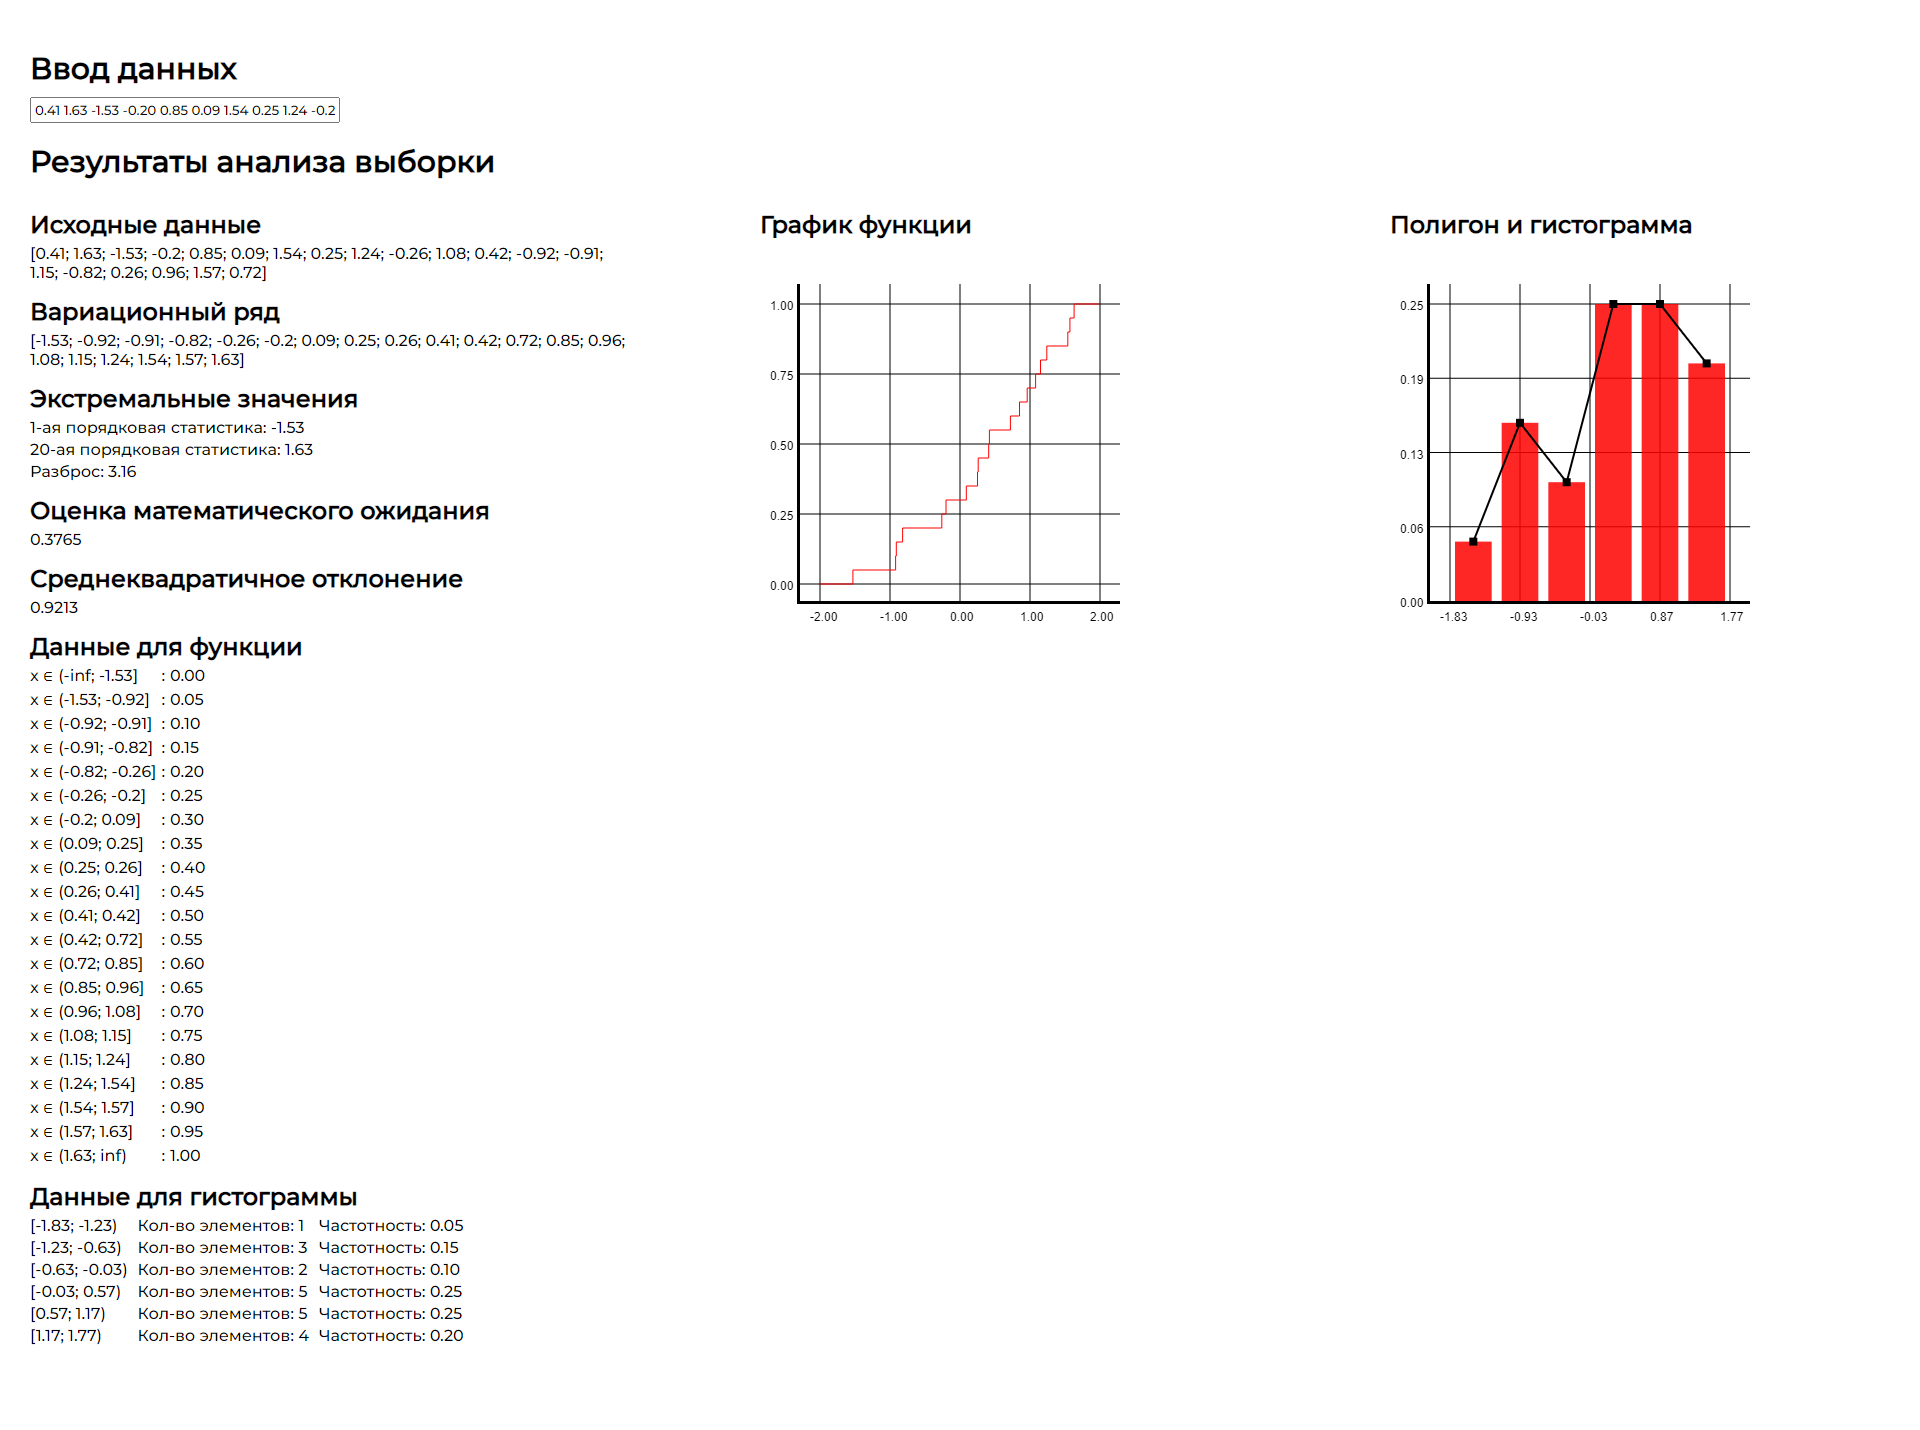
\includegraphics[width=15cm]{screenshot.png}
\end{center}
\end{document}